\documentclass[12pt]{article}
\usepackage[a4paper, left=3.17cm, right=3.17cm, top=2.54cm, bottom=2.54cm]{geometry}
\usepackage[UTF8]{ctex}
\usepackage{newtxtext,newtxmath}
\usepackage{amsmath}
\usepackage{amsfonts}
\usepackage{chemformula}
\usepackage{cite}
\usepackage[colorlinks, linkcolor=black, anchorcolor=black, citecolor=black]{hyperref}
\usepackage{graphicx}
\usepackage{subfigure}
\usepackage{makecell}
\usepackage{caption}
\usepackage{booktabs}
\usepackage{abstract}
\usepackage{longtable}
\usepackage{diagbox}
\usepackage{float}

\renewcommand{\abstractname}{\Large\textbf{摘要}}

\setlength{\parskip}{0.5em}
\title{数字频率计}
\author{\textup{廖章盛}}
\begin{document}

\begin{titlepage}
    \setcounter{page}{0}
    \newcommand{\HRule}{\rule{\linewidth}{0.5mm}}
    \centering
    
\includegraphics[width=8cm]{../DHU.png}\\[1cm]
    \quad\\[1.5cm]
    \textsl{\Large 东华大学 }\\[0.5cm]
    \textsl{\large 课程设计报告}\\[0.5cm]

    \makeatletter
    \HRule \\[0.4cm]
    { \huge \bfseries \@title}\\[0.4cm]
    \HRule \\[1.5cm]
    {\large
    \begin{tabular}{c@{~~}c}
        \makebox[2em][s]{专业}: & \underline{\makebox[8em][c]{专业}} \\
        \makebox[2em][s]{姓名}: & \underline{\makebox[8em][c]{姓名}}     \\
        \makebox[2em][s]{学号}: & \underline{\makebox[8em][c]{学号}}  \\
    \end{tabular}\\[1cm]}
    \makeatother
    {\large \today}\\[2cm]
    \vfill
\end{titlepage}

\begin{abstract}
    随着科技的不断发展,数字式频率计的应用前景越来越广泛,在物联网、智能家居、医疗设备等领域都有着广泛的应用。本次课程设计主要基于FPGA和数字电路设计了一个简易的数字频率计。

    本数字频率计数器主要由分频、计数、锁存、译码显示等主要模块构成。由这些模块组合成整体电路。

    分频模块:输入10MHz的时钟信号,经过分频后,可输出1MHz、100KHz、10KHz、1KHz、100Hz、10Hz、1Hz、0.1Hz的信号,用于后续的调试信号。

    计数模块:计数模块是一个10000进制计数器,输入的时钟信号为分频模块输出的信号,经过计数后,可以获得四位的计数结果。

    锁存模块:两个八位锁存器对计数模块输出四位计数结果进行锁存,锁存后的信号送入译码显示模块。

    译码显示模块:锁存模块输出四位数据到数据选择器,数据选择器选择一位数据输出,再送入译码器,译码器输出对应的七段显示码,最后送入数码管,显示出来。
    \par\textbf{关键词:}数字电路;频率计;FPGA
\end{abstract}

\newpage
\tableofcontents

\section{设计概述}

在生产实践和科学实验中,经常需要测量信号的频率或周期。数字频率计和数字周期计就是用数字方式测量和显示被测信号频率或周期的仪器。数字测频和数字测周的原理是相似的,所以测频仪器一般兼有测周功能。实用的数字频率计或周期计可以测量多种不同形式的周期性波形,如正弦波、三角波、方波等。

本设计的目的在于帮助读者理解频率测量和周期测量的基本原理以及计数型测量仪表的量程扩展方法,所以只要求对输入为TTL方波信号进行测量。

\section{设计任务及要求}

\subsubsection*{基本任务}

要求设计一个测量TTL方波信号频率或周期的数字系统。用按键选择测量信号频率或周期。测量值采用4个LED七段数码管显示,并以发光二极管指示测量对象:频率(周期)以及测量值的单位:Hz(s)、kHz(ms)。频率和周期的测量范围都有4档量程。

\subsubsection*{要求}

\begin{enumerate}
    \item 测量结果显示四位有效数字,测量精度为万分之一。
    \item 测量范围:频率0.1Hz~999.9KHz,分为4档。
          \begin{itemize}
              \item 第一档:100.0 Hz~999.9 Hz
              \item 第二档:1.000 kHz~9.999 kHz
              \item 第三档:10.00 kHz~99.99 kHz
              \item 第四档:100.0 kHz~999.9 kHz
          \end{itemize}


          周期测量范围:0.1 us-999.9 ms,分为4档。
          \begin{itemize}
              \item 第一档:1.000 ms~9.999 ms
              \item 第二档:10.00 ms~99.99 ms
              \item 第三档:100.0 ms~999.9 ms
              \item 第四档:1.000 s~9.999 s
          \end{itemize}


    \item 量程切换可以采用两个按键手动切换或由电路控制自动切换。
    \item 设计一个周期性方波产生电路输出频率/周期计调试所需的信号。输出信号的频率范围与测量范围相同,分为4个量程。再设置4个按键在每档范围内选择4位有效数字的9~16个固定频率,最高位数值必须分布为1~9,信号占空比可以任意。

\end{enumerate}

\section{系统概述}

\subsection{设计思想}

\begin{itemize}
    \item 数字频率计的基本原理是测量周期性信号在单位时间内的信号周波数,所以它的主要电路是计数器,需要控制的是计数器的输入脉冲和计数时间,其输入脉冲为被测信号,计数时间为时基信号的周期(单位时间)。
    \item 被测信号的频率就是在单位时间内所产生的脉冲个数。因此可以利用计数器来完成计数功能,在利用公式$f=\frac{N}{T}$就可以计算出待测信号的频率。
    \item 计数器进行计数,利用锁存器将计数的结果进行锁存,并把锁存的结果输送到译码器来控制七段显示器显示输出结果。同时还需用一个逻辑控制电路产生相应的锁存和清零信号以分别控制锁存器和计数器的工作状态。
\end{itemize}

\subsection{可行性论证}

\begin{itemize}
    \item 频率的物理意义是单位时间(1s)内信号的周波数。所以频率测量问题等同于时间测量问题。
    \item 在电子系统中,频率、周期、时间的测量通常采用计数器。
    \item 计数测量一般采用比较法:
          \begin{enumerate}
              \item 测量一段标准时间内周期性信号的周波数(测频)。
              \item 计数器的计数时间(开门时间)和计数脉冲是关键参数。
          \end{enumerate}
\end{itemize}

\subsection{各功能组成}

\begin{enumerate}
    \item 产生系统基准时钟的石英晶体振荡器;
    \item 多级分频电路;
    \item 计数锁存电路;
    \item 显示译码电路;
    \item 锁存清零驱动电路;
    \item 量程切换控制;
    \item 小数点位置控制;
    \item 测量时基控制;
\end{enumerate}

\subsection*{总体系统框图}

总体系统框图如图\ref*{fig:system}。

\begin{figure}[H]
    \centering
    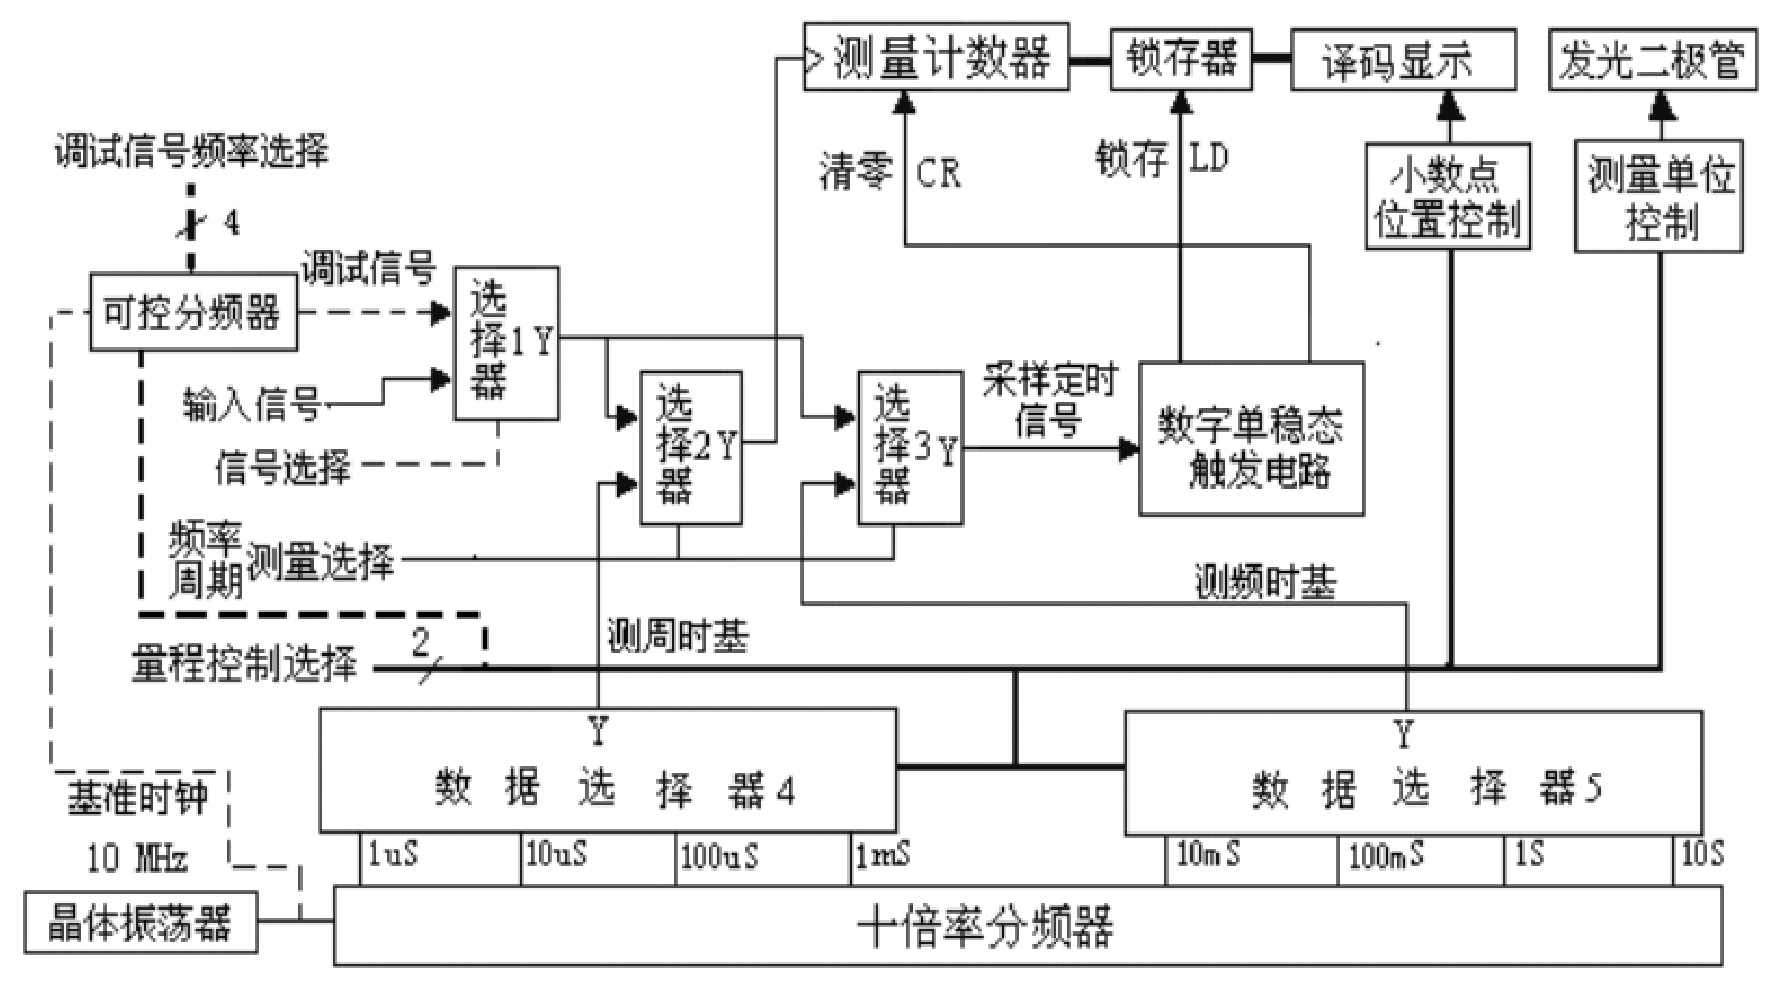
\includegraphics[width=1\textwidth]{./fig/system.png}
    \caption{总体系统框图}
    \label{fig:system}
\end{figure}

\newpage
\section{模块设计}

\subsection{八级十分频电路}

十分频电路如图\ref*{fig:div8},它是由一个二-五-十进制计数器构成,输入频率接CLKA口,输出的QD接CLKB口,这样每隔10个输入上升沿,就会输出1个上升沿,达成十分频的效果。八级十分频电路由八片十分频级联而成。

\begin{figure}[H]
    \centering
    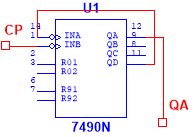
\includegraphics[width=0.6\textwidth]{./fig/div8.jpg}
    \caption{八级十分频电路}
    \label{fig:div8}
\end{figure}

\subsection{四位数码管译码显示电路}

四位数码管译码显示电路如图\ref*{fig:4scan}。此电路由一片74161加法计数器、五片74153四选一数据选择器、一片7448七段译码器构成。

74161时钟信号端接入一个1KHz的信号,可以使得四位数码管扫描速度超过人眼分辨能力,从而达到静止显示的效果。74161输出两位二进制数,分别接入两片74153的A、B,每次选择一位数据输出,构成一个BCD码,再接入7448译码器,输出对应的七段显示码,最后接入四位数码管,显示出来。

\begin{figure}[H]
    \centering
    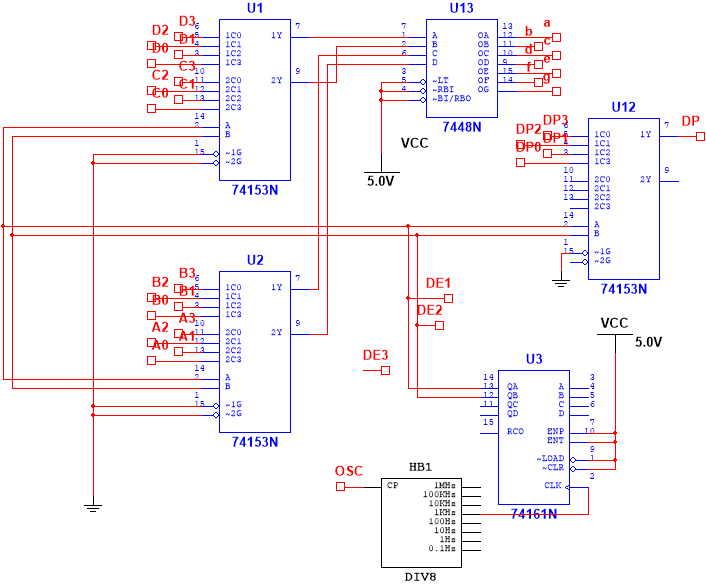
\includegraphics[width=0.8\textwidth]{./fig/4scan.png}
    \caption{四位数码管译码显示电路}
    \label{fig:4scan}
\end{figure}

\subsection{计数锁存电路}

计数锁存电路如图\ref*{fig:countLatch}。此电路由四片74160加法计数器、两片74374锁存器、四位数码管译码显示电路构成。

四片74160级联构成一个10000进制的加法计数器,输出的数据接入两片74374锁存器进行锁存,锁存器的输出接入四位数码管译码显示电路。

在一个测量周期内,计数器进行计数,锁存器接收到锁存信号后进行锁存,之后计数器立马接收到清零信号,进行清零,再次开始计数。这样就可以在一个测量周期内完成计数、锁存、清零的过程,从而达到测量频率的目的。

锁存器内锁存的数据送入四位数码管译码显示电路,译码显示电路每次将选择一位数据进行显示。由于译码显示电路的扫描速度很快,所以人眼看到的是四位数码管同时显示的效果。

\begin{figure}[H]
    \centering
    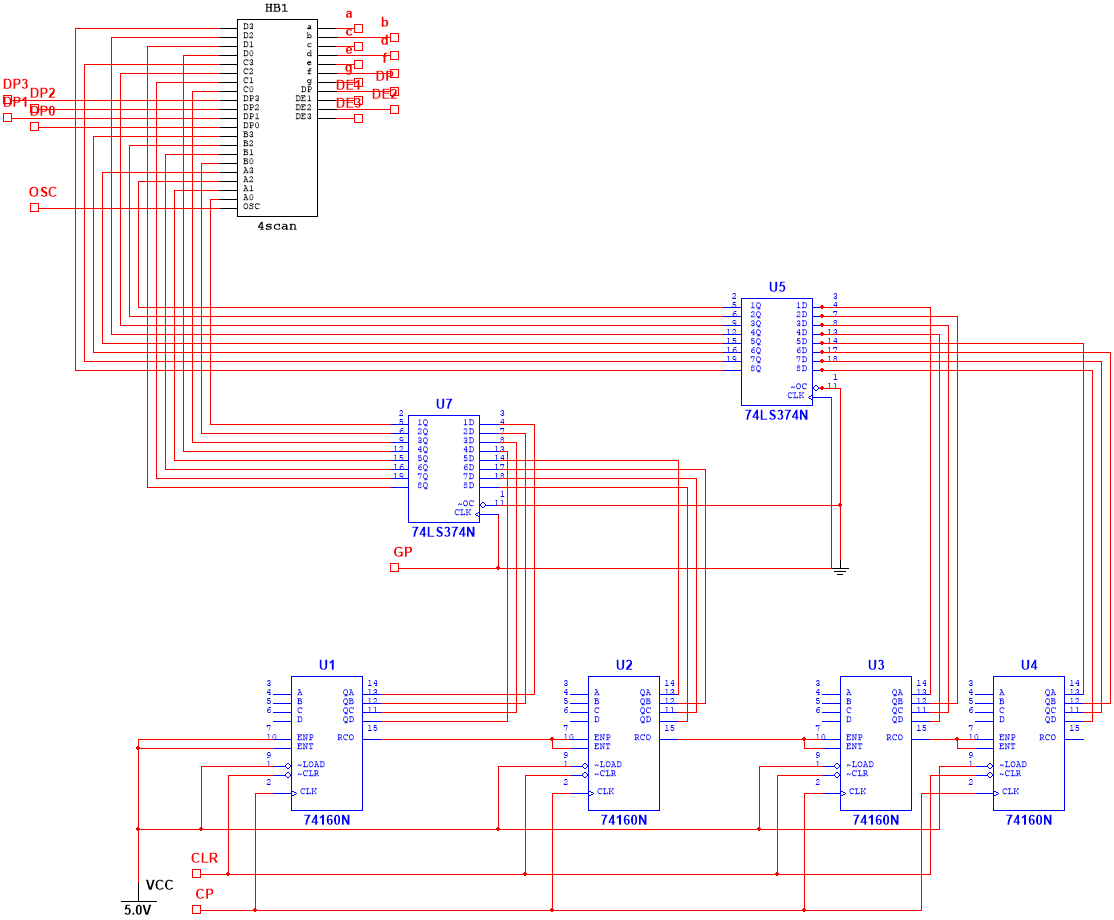
\includegraphics[width=0.8\textwidth]{./fig/countLatch.png}
    \caption{计数锁存电路}
    \label{fig:countLatch}
\end{figure}

\subsection{单稳态触发电路}

单稳态触发电路如图\ref*{fig:monostable}。此电路由三个D触发器与一些逻辑门构成。单稳态触发电路的波形如图\ref*{fig:monostableWave}。时钟信号CP频率非常高时,输出的信号Y、CLR的周期为输入信号M的周期。且Y信号比CLR信号超前一个正半周,所以输出的Y、CLR信号可以分别接入计数锁存电路的锁存器锁存信号、计数器清零信号,使得可以在锁存之后立即清零,提高测量精度。

\begin{figure}[H]
    \centering
    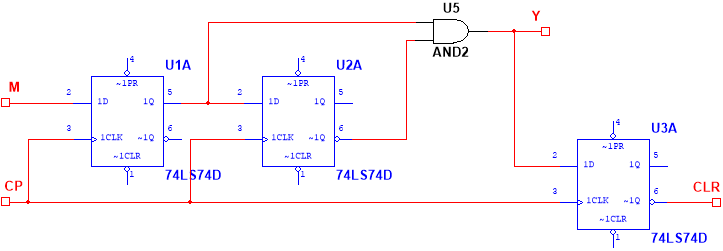
\includegraphics[width=0.8\textwidth]{./fig/monostable.png}
    \caption{单稳态触发电路}
    \label{fig:monostable}
\end{figure}

\begin{figure}[H]
    \centering
    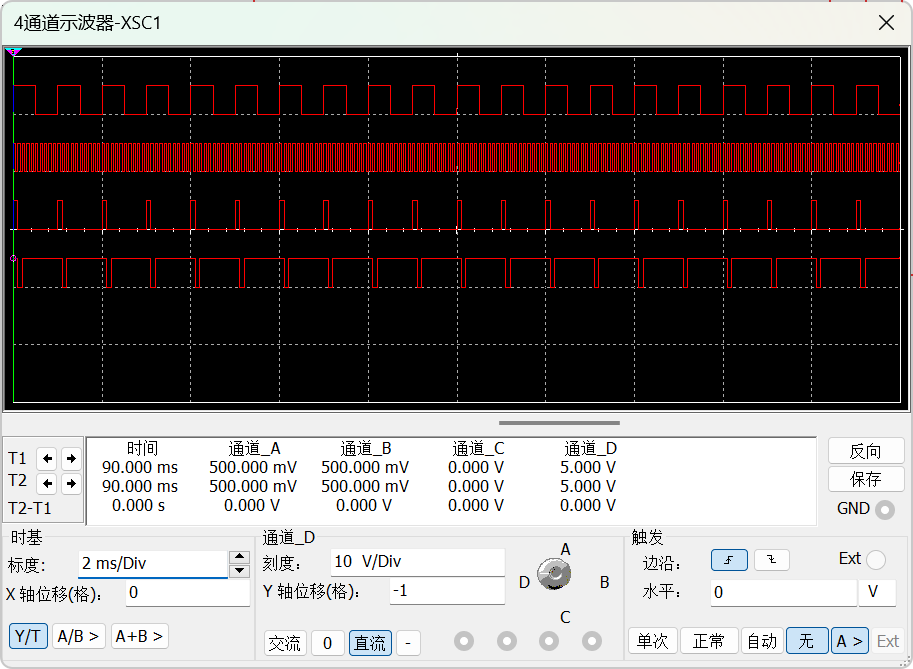
\includegraphics[width=0.8\textwidth]{./fig/monostableWave.png}
    \caption{单稳态触发电路输出波形}
    \label{fig:monostableWave}
\end{figure}

\subsection{小数点控制电路}

小数点控制电路如图\ref*{fig:dot}。此电路由一些逻辑门构成,输入$A_1A_0$两位二进制数,对应显示第一、第三、第二、第一位小数点,最后一位小数点默认不显示。对应的逻辑真值表如表\ref*{tab:dot}。

\begin{figure}[H]
    \centering
    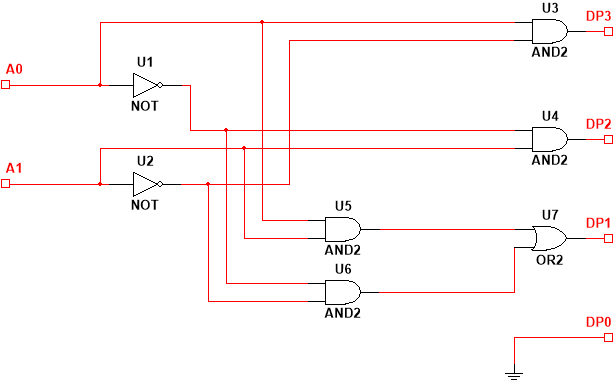
\includegraphics[width=0.8\textwidth]{./fig/dot.png}
    \caption{小数点控制电路}
    \label{fig:dot}
\end{figure}

\begin{table}
    \centering
    \caption{小数点控制电路逻辑真值表}
    \label{tab:dot}
    \begin{tabular}{|c|c|c|c|c|}
        \hline
        \diagbox{输入$A_1A_0$}{输出} & $DP_3$ & $DP_2$ & $DP_1$ & $DP_0$ \\ \hline
        00                    & 0     & 0     & 1     & 0     \\ \hline
        01                    & 1     & 0     & 0     & 0     \\ \hline
        10                    & 0     & 1     & 0     & 0     \\ \hline
        11                    & 0     & 0     & 1     & 0     \\ \hline
    \end{tabular}
\end{table}

\subsection{测量时基选择电路}

测量时基选择电路如图\ref*{fig:timebase}。此电路由一片四选一数据选择器和八级十分频电路构成。四选一数据选择器的$D_0$、$D_1$、$D_2$、$D_3$分别接入八级十分频电路的100Hz、10Hz、1Hz、0.1Hz输出端,分别对应0.01s、0.1s、1s、10s的时基信号,选择器的A、B用于选择测量时基。

\begin{figure}[H]
    \centering
    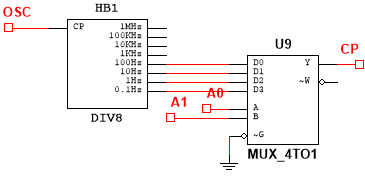
\includegraphics[width=0.8\textwidth]{./fig/timebase.png}
    \caption{测量时基选择电路}
    \label{fig:timebase}
\end{figure}

\subsection{调试信号选择电路}

调试信号选择电路如图\ref*{fig:signal}。此电路由一片四选一数据选择器、八级十分频电路、74160计数器构成。四选一数据选择器的$D_0$、$D_1$、$D_2$、$D_3$分别接入八级十分频电路的1MHz、100KHz、10KHz、1KHz输出端,对应要测量的频率。选择器的A、B用于选择测量信号。选择的信号接入74160计数器,进行分频,分频的级数由ABCD端接入的预置数控制,为$10-(DCBA)_{BCD}$级分频。

\begin{figure}[H]
    \centering
    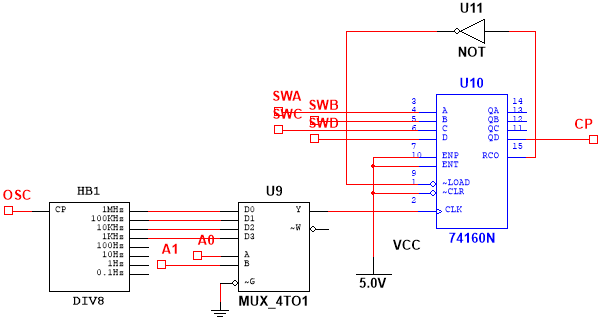
\includegraphics[width=0.8\textwidth]{./fig/signal.png}
    \caption{调试信号选择电路}
    \label{fig:signal}
\end{figure}

\section{电路组构与调试}

将各部分封装成符号文件,组装。在Quartus II中进行仿真,分配引脚,下载到FPGA中进行调试。

总电路图如图\ref*{fig:total}。各个模块封装成的符号文件如图\ref*{fig:symbol}。

\subsection{遇到的问题}

\begin{enumerate}
    \item 显示数据错误。
    \item 小数点显示错位。
\end{enumerate}

\subsubsection*{现象记录及原因分析}

\begin{enumerate}
    \item 显示数据错误。经过检查,发现是由于信号调试模块的分频计数器使用错误(本该使用74160,结果用了74161,导致分频混乱,最终使结果错误)。
    \item 纠正完数据显示错误的原因后,发现第二、第三个数码管显示的数据反了。经过检查,发现是由于引脚分配错误,导致数码管译码显示错误,造成相应数码管错位。
\end{enumerate}

\subsection{解决方案}

\begin{enumerate}
    \item 更换分频计数器。将74161用74160替换,再连接相应的电路。进行仿真,发现数据显示部分正确。
    \item 调换PIN\_41、PIN\_42引脚后,数据显示全部正确。
\end{enumerate}

\subsection{功能的测试方法、步骤、设备、记录的数据}

\subsubsection*{功能测试方法}

\begin{enumerate}
    \item 按键SW1、SW2可以控制小数点、单位的显示、测量时间、量程的切换、最小误差。
    \item SW3、SW4、SW5、SW6对输入频率进行分频级别调试(可进行$1 \sim 10$分频)。
    \item $0 \sim 3$号数码管进行四位数据显示。
    \item 第一个LED用于单位显示,灯亮表示KHz,灯灭表示Hz。
\end{enumerate}

\subsubsection*{功能测试步骤}

\begin{itemize}
    \item 分析与综合、编译总电路文件。
    \item 将总电路文件下载到FPGA中。LP-2900灯亮,开始测试:
    \begin{enumerate}
        \item 同时按下SW1、SW2,表示选择测量量程为100.0KHz~999.9KHz、小数点位置为第三位、误差为100Hz、测量时间为0.01s。
        \item 按下SW6,表示分频级别为$10-(1000)_{BCD} = 2$。
    \end{enumerate}
    \item 预期结果:$f = \frac{1MHz}{2} = 500.0 KHz$。测量结果如图\ref*{fig:test},显示为500.0KHz。表明电路工作正常。
\end{itemize}

\begin{figure}[H]
    \centering
    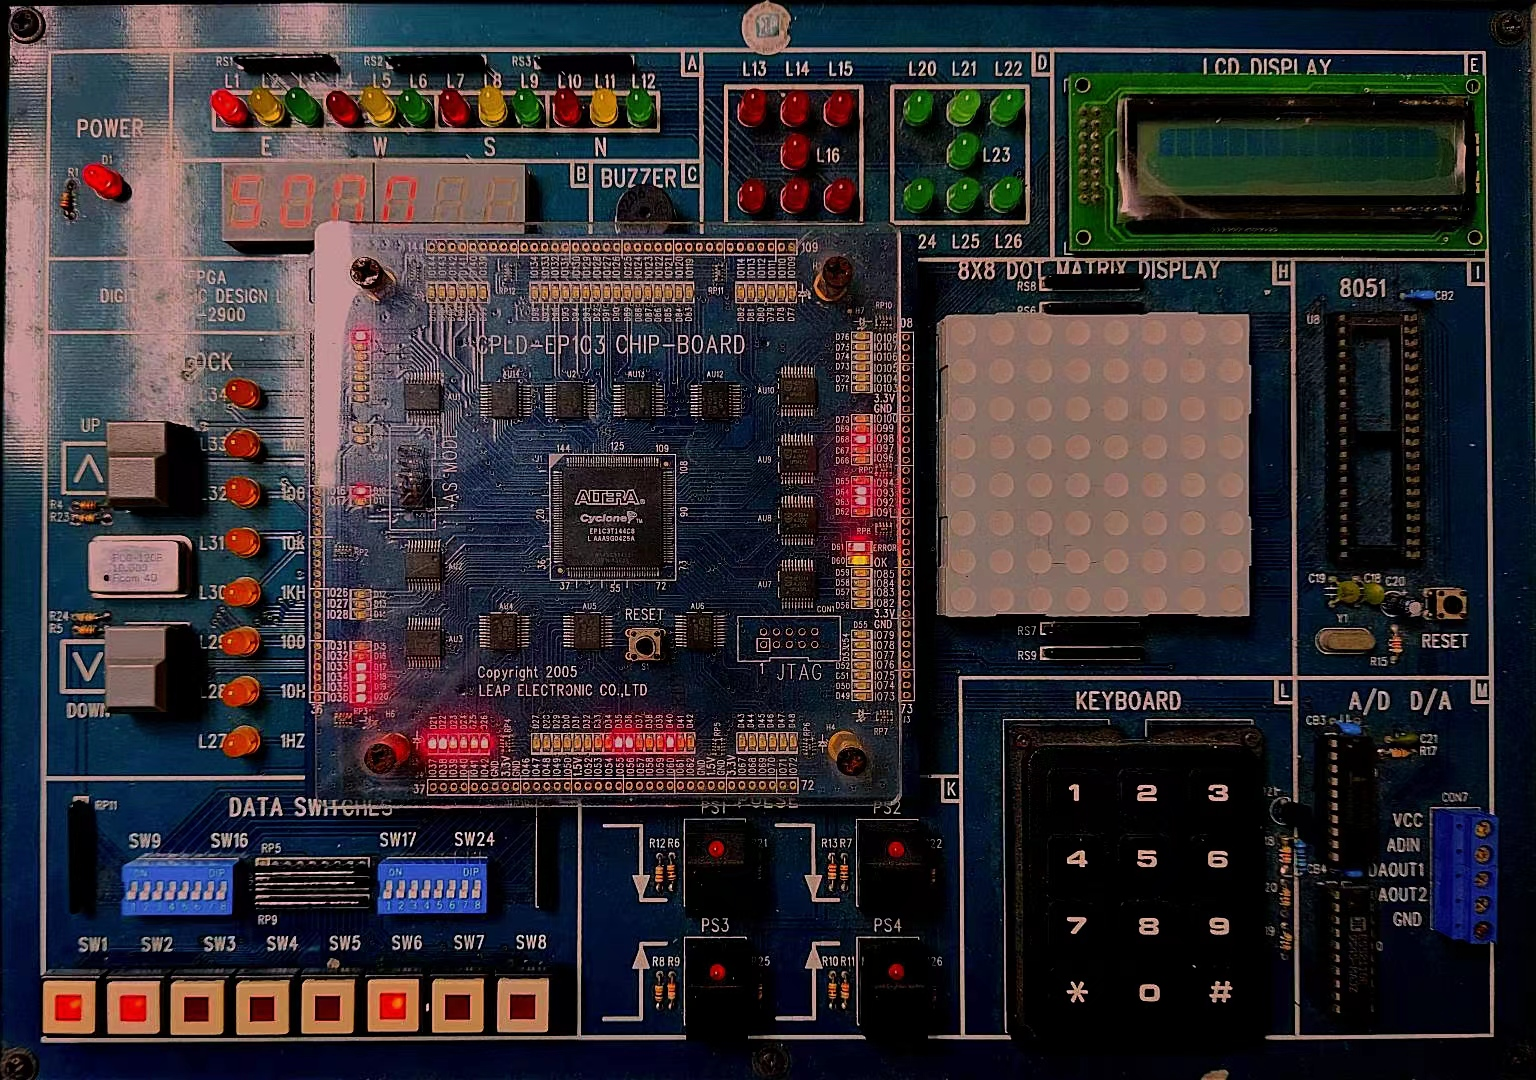
\includegraphics[width=1\textwidth]{./fig/test.jpg}
    \caption{测量结果}
    \label{fig:test}
\end{figure}

\subsubsection*{功能测试设备}

Quartus II 软件、LP-2900开发板。

\subsubsection*{记录数据}

测量的数据如表\ref*{tab:data}

\begin{table}[H]
    \centering
    \caption{测量数据}
    \label{tab:data}
    \resizebox{\textwidth}{!}{
        \begin{tabular}{|c|c|c|c|c|c|c|c|c|c|c|} \hline
            \diagbox{范围}{分频}{结果} & 1   & 2        & 3       & 4  & 5        & 6       & 7  & 8        & 9       & 10 \\ \hline
            100.0Hz~999.9Hz   & 999.9 & 500.0 & 333.3 & 250.0 & 200.0 & 666.7 & 142.8 & 125.0 & 111.1 & 100.0 \\ \hline
            1.000KHz~9.999KHz & 9.999 & 5.000 & 3.333 & 2.500 & 2.000 & 6.667 & 1.428 & 1.250 & 1.111 & 1.000 \\ \hline
            10.00KHz~99.99KHz & 99.99 & 50.00 & 33.33 & 25.00 & 20.00 & 66.67 & 14.28 & 12.50 & 11.11 & 10.00 \\ \hline
            100.0KHz~999.9KHz & 999.9 & 500.0 & 333.3 & 250.0 & 200.0 & 666.7 & 142.8 & 125.0 & 111.1 & 100.0 \\ \hline
        \end{tabular}}
\end{table}

测量的数据与预期结果相符,测量百分误差在0.1\%以内。表明电路工作正常。

\newpage
\section{总结与体会}

\subsection{完成情况}

截至第10周,笔者已顺利地完成了本次课程设计的基础内容,且测量结果较为准确。

\subsection{心得体会}

在这次数字频率计课程设计中,我学到了很多关于数字电路、电路设计、仿真软件的使用等方面的知识。通过这个课程设计,我不禁掌握了这些知识,还深入了解如何运用这些知识来解决问题。

我认为我在以下几个方面取得了收获:

\begin{itemize}
    \item 掌握了数字电路的基本知识,学会频率计算的方法。
    \item 电路设计及软件的使用技巧。
    \item 增强了解决实际问题的能力。
\end{itemize}

同时,我也发现了一些问题:电路布局不够优美、电路设计不够简洁、电路设计不够完善等。这些问题将在今后的学习中得到改善。

\newpage
\nocite{*}
\bibliographystyle{plain}
\begin{thebibliography}{99}

    \bibitem{ref1}童诗白, 华成英. 《模拟电子技术基础(第五版)》. 高等教育出版社, 2015.
    \bibitem{ref2}崔葛瑾, 沈利芳, 李伟民. 《基于FPGA的数字电路系统设计》. 西安电子科技大学出版社. 2008.7.

\end{thebibliography}

\newpage
\section*{附录}

\subsection*{封装符号图}

\begin{figure}[H]
    \centering
    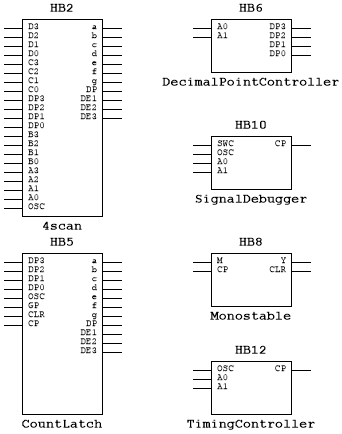
\includegraphics[width=1\textwidth]{./fig/symbol.png}
    \caption{封装符号图}
    \label{fig:symbol}
\end{figure}

\subsection*{总电路图}

\begin{figure}[H]
    \centering
    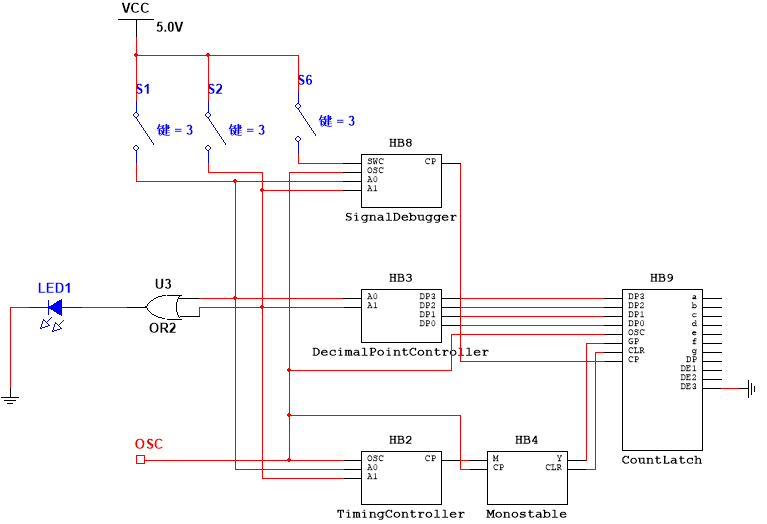
\includegraphics[width=1\textwidth]{./fig/total.png}
    \caption{总电路图}
    \label{fig:total}
\end{figure}



\end{document}
